\chapter{Genes and DNA}\label{ch:g9:genes-and-dna}

The \omterm{def:g9:chromosomes:chromosomes}{chromosomes} carry the determinants --- but a thread is
not yet a text. What, along a \omterm{def:g9:chromosomes:chromosomes}{chromosome}, \emph{is} one
determinant? And what is the thread made of, that a \omterm{def:g6:cell-unit-of-life:parts}{nucleus}
thousandths of a millimetre wide can hold instructions for a
whole human being
(\cref{exo:g9:heredity-and-traits:12})? Two names answer,
and they are the most famous in modern \omterm{def:g1:living-or-not:living}{biology}: the \omterm{def:g9:genes-and-dna:gene}{gene},
and \omterm{def:g9:genes-and-dna:dna}{DNA}.

\section{Genes: the determinants, located}

\begin{definition}[Gene and alleles]\label{def:g9:genes-and-dna:gene}
A \emph{gene}\index{gene} is one determinant made precise:
a \emph{segment of a \omterm{def:g9:chromosomes:chromosomes}{chromosome}} carrying the instructions
for one \omterm{def:g9:heredity-and-traits:traits}{trait}'s piece of the build --- one gene for the
blood-group machinery, others for eye-color pigments,
thousands upon thousands along the 46 threads, each at its
fixed address. A gene can exist in several versions ---
\emph{alleles}\index{allele}: the blood-group gene's A, B
and O versions, the eye-color gene's brown and blue. Same
address, different spelling.
\end{definition}

\begin{proposition}[Two copies, and what showing means]\label{prop:g9:genes-and-dna:twocopies}
\omterm{def:g9:chromosomes:chromosomes}{Chromosomes} come in pairs
(\cref{prop:g9:chromosomes:counts}) --- so every \omterm{def:g9:genes-and-dna:gene}{gene}
comes in \emph{two copies}, one per partner, one from each
parent. The copies may be the same \omterm{def:g9:genes-and-dna:gene}{allele} or different;
when different, one may be \emph{expressed} and the other
carried silent --- and the family album's mysteries
resolve into mechanism:
\begin{itemize}
  \item carriage-without-showing
        (\cref{ex:g9:heredity-and-traits:skip}): the
        silent \omterm{def:g9:genes-and-dna:gene}{allele} rides the second partner;
  \item the group-O child of A- and B-parents
        (\cref{pb:g9:heredity-and-traits:1}): each parent
        carried O silent, and the halving dealt both O's
        together;
  \item the blue-eyed child of brown-eyed parents: two
        silent blues, meeting --- one chance in four, when
        both parents carry one each: the halving deals
        each parent's blue with one chance in two, and the
        two deals are independent.
\end{itemize}
\end{proposition}
\admitted

\begin{example}[Blood groups, fully mechanized]\label{ex:g9:genes-and-dna:bloodgroups}
One \omterm{def:g9:genes-and-dna:gene}{gene}, three \omterm{def:g9:genes-and-dna:gene}{alleles}, two copies per person: A with A
or O shows group A; B with B or O shows B; A with B shows
AB (both expressed --- \omterm{def:g9:genes-and-dna:gene}{alleles} are not always
silencable); O with O shows O. The donation register's
whole pattern --- including every ``surprise'' --- is the
arithmetic of two-copy deals.
\end{example}

\section{DNA: what the text is written in}

\begin{definition}[DNA]\label{def:g9:genes-and-dna:dna}
Chemically, a \omterm{def:g9:chromosomes:chromosomes}{chromosome} is one immensely long, coiled
molecule of \emph{DNA}\index{DNA} (with packing proteins):
a double strand --- the famous twisted ladder --- whose
rungs are pairs of four chemical letters. \emph{The order
of the letters along the strand is the information}: a
\omterm{def:g9:genes-and-dna:gene}{gene} is a stretch of that sequence, as a sentence is a
stretch of a page. Four letters, three billion of them in
one human deck --- enough text for a build's whole
instruction set, coiled into every \omterm{def:g6:cell-unit-of-life:parts}{nucleus}.
\end{definition}

\begin{example}[Seeing it yourself]\label{ex:g9:genes-and-dna:extraction}
\omterm{def:g9:genes-and-dna:dna}{DNA} is kitchen-extractable: mash a banana or an onion,
add salty water and a little washing-up liquid (\omterm{def:g6:cell-unit-of-life:parts}{membranes}
undone --- \cref{def:g6:cell-unit-of-life:parts}'s
envelopes are its target), strain, and layer cold spirit
on top: at the boundary rises a tangle of whitish
threads, spoolable on a toothpick. Those threads are \omterm{def:g9:genes-and-dna:dna}{DNA}
--- the actual molecule of this chapter, in actual
centimetres.
\end{example}

\begin{omfigure}
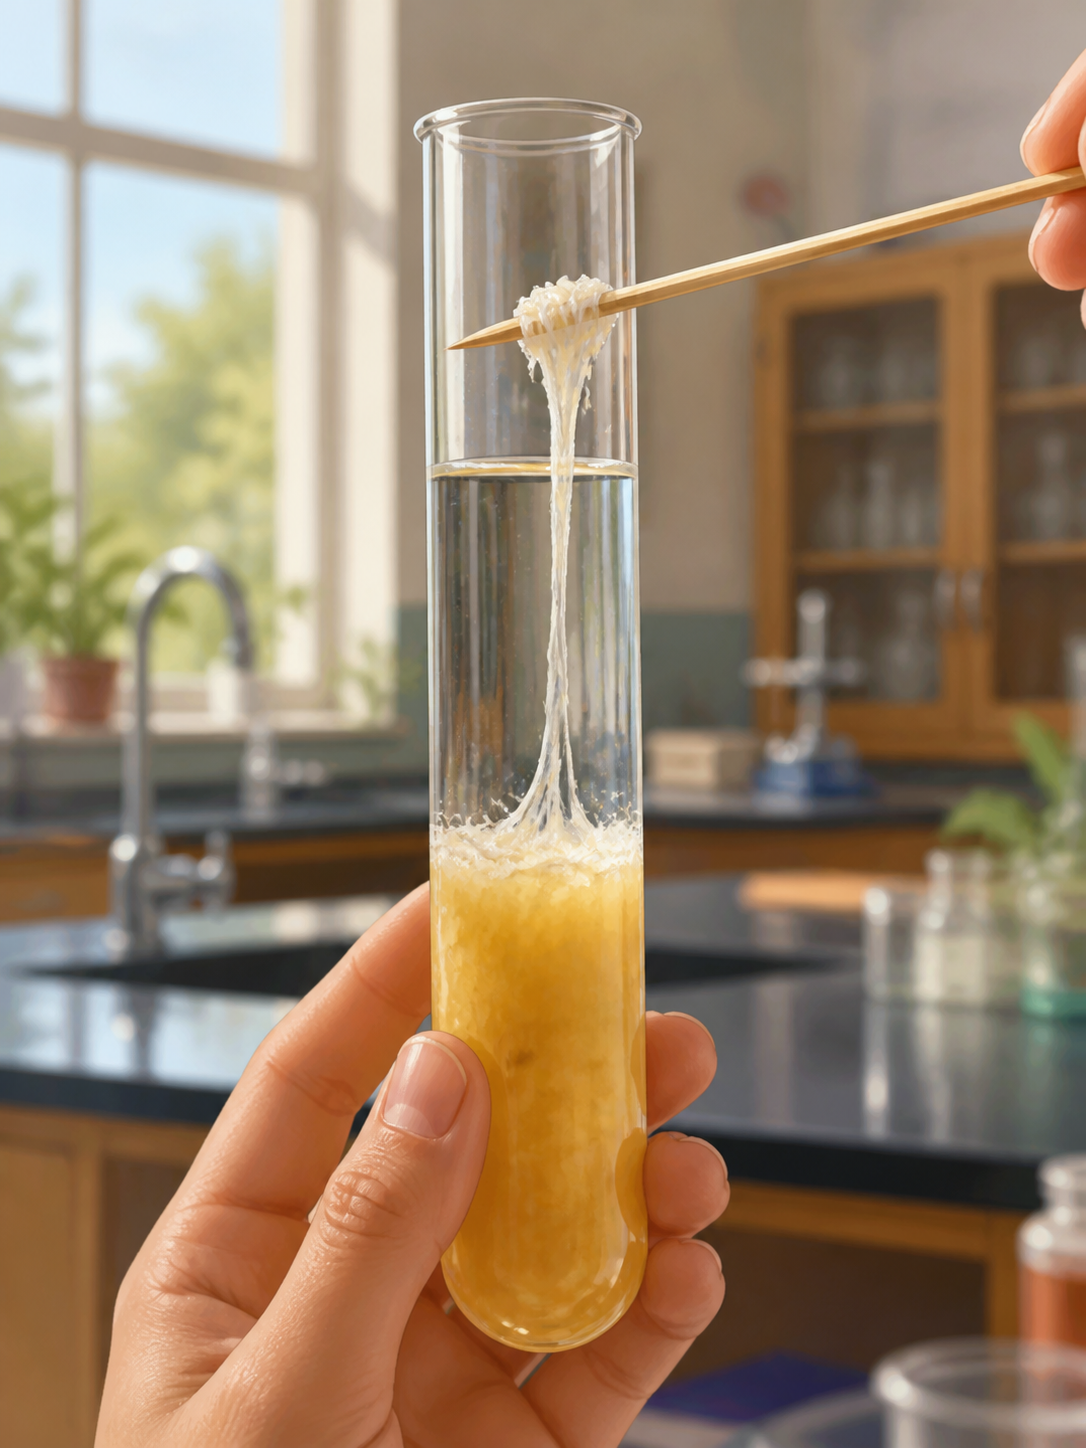
\includegraphics[width=0.42\linewidth]{images/book1/ai/g9-dna-extraction.png}

{\small The kitchen extraction's payoff: the molecule of
\omterm{def:g9:heredity-and-traits:heredity}{heredity}, spooled on a stick.}
\end{omfigure}

\begin{proposition}[What DNA's structure explains]\label{prop:g9:genes-and-dna:explains}
The double strand is not decoration --- each property
answers an old question:
\begin{itemize}
  \item \emph{copying}
        (\cref{prop:g5:first-look-at-cells:growth}'s
        faithful divisions): the two strands are
        letter-by-letter complements, so pulled apart,
        each rebuilds its partner --- one ladder becomes
        two identical ladders, one per daughter \omterm{def:g5:first-look-at-cells:cell}{cell};
  \item \emph{\omterm{def:g9:genes-and-dna:gene}{alleles}}: versions of a \omterm{def:g9:genes-and-dna:gene}{gene} are small
        spelling differences in the sequence ---
        same address, changed letters;
  \item \emph{mutation}\index{mutation}: copying is
        near-perfect, not perfect --- a rare miscopied
        letter creates a \emph{new} \omterm{def:g9:genes-and-dna:gene}{allele}. Mostly
        neutral, sometimes harmful, occasionally useful:
        \omterm{prop:g9:genes-and-dna:explains}{mutation} is where fresh spellings, and ultimately
        all \omterm{def:g9:genes-and-dna:gene}{alleles}, come from --- the raw novelty
        \cref{ch:g9:how-species-change} will need;
  \item \emph{reading}: a \omterm{def:g5:first-look-at-cells:cell}{cell} uses a \omterm{def:g9:genes-and-dna:gene}{gene} by reading its
        sequence and building the corresponding working
        molecule --- and each \omterm{def:g5:first-look-at-cells:cell}{cell} kind reads its own
        selection of the library:
        \cref{exo:g9:chromosomes:12}'s puzzle, resolved
        as promised.
\end{itemize}
\end{proposition}
\admitted

\begin{remark}[One code, all of life]\label{rem:g9:genes-and-dna:universal}
The deepest fact comes last: \emph{every} \omterm{def:g6:exploring-our-environment:components}{living thing}
writes its \omterm{def:g9:genes-and-dna:gene}{genes} in the same \omterm{def:g9:genes-and-dna:dna}{DNA} letters and reads them by
the same code --- oak, \omterm{ex:g6:producing-our-food:bread}{yeast}, whale, the \omterm{def:g6:producing-our-food:fermentation}{microbes} of
\cref{ch:g6:producing-our-food}, you. This is the \omterm{prop:g5:first-look-at-cells:principle}{unity of
life} (\cref{prop:g5:first-look-at-cells:principle}) at its
foundation, and the \omterm{prop:g6:classification-kinship:kinship}{kinship} tree's
(\cref{rem:g6:classification-kinship:implies}) strongest
evidence yet: a shared language argues a shared origin.
It is also why genetic engineering works at all --- a \omterm{def:g9:genes-and-dna:gene}{gene}
moved between \omterm{def:g5:biodiversity:species}{species} is still readable, as a sentence
photocopied into another book.
\end{remark}

\begin{method}[The three-level reading]\label{met:g9:genes-and-dna:levels}
Any \omterm{def:g9:heredity-and-traits:heredity}{heredity} question can now be read at three levels ---
practice switching:
\begin{enumerate}
  \item \emph{family level}: who shows, who carries, who
        transmits (\cref{ch:g9:heredity-and-traits});
  \item \emph{\omterm{def:g9:chromosomes:chromosomes}{chromosome} level}: which threads, halved and
        restored, carry the deal
        (\cref{ch:g9:chromosomes});
  \item \emph{molecule level}: which \omterm{def:g9:genes-and-dna:gene}{gene}, which \omterm{def:g9:genes-and-dna:gene}{alleles},
        what spelling --- and, for a new \omterm{def:g9:heredity-and-traits:traits}{trait}, what
        \omterm{prop:g9:genes-and-dna:explains}{mutation}.
\end{enumerate}
One story, three magnifications; an answer is complete
when it runs at all three.
\end{method}

\section{Exercises}

\begin{exercise}[$\star$]\label{exo:g9:genes-and-dna:1}
Define \omterm{def:g9:genes-and-dna:gene}{gene} and \omterm{def:g9:genes-and-dna:gene}{allele}, with the blood-group example.
\end{exercise}

\begin{exercise}[$\star$]\label{exo:g9:genes-and-dna:2}
Why does every \omterm{def:g9:genes-and-dna:gene}{gene} come in two copies, and where do they
sit?
\end{exercise}

\begin{exercise}[$\star$]\label{exo:g9:genes-and-dna:3}
What is \omterm{def:g9:genes-and-dna:dna}{DNA}'s information, physically? How many letters,
of how many kinds, in a human deck?
\end{exercise}

\begin{exercise}[$\star$]\label{exo:g9:genes-and-dna:4}
How does the double strand make faithful copying
possible?
\end{exercise}

\begin{exercise}[$\star$]\label{exo:g9:genes-and-dna:5}
What is a \omterm{prop:g9:genes-and-dna:explains}{mutation}, and what are its three possible
characters?
\end{exercise}

\begin{exercise}[$\star$]\label{exo:g9:genes-and-dna:6}
State \cref{rem:g9:genes-and-dna:universal}'s fact and
its two consequences.
\end{exercise}

\begin{exercise}[$\star\star$]\label{exo:g9:genes-and-dna:7}
Mechanize the blue-eyed child of brown-eyed parents:
copies, deals, and the one-in-four.
\end{exercise}

\begin{exercise}[$\star\star$]\label{exo:g9:genes-and-dna:8}
Work \cref{ex:g9:genes-and-dna:bloodgroups}: list the
\omterm{def:g9:genes-and-dna:gene}{allele} pairs behind each of the four groups.
\end{exercise}

\begin{exercise}[$\star\star$]\label{exo:g9:genes-and-dna:9}
Resolve \cref{exo:g9:chromosomes:12} in this chapter's
terms: what does a \omterm{def:g8:nervous-communication:neuron}{neuron} read that a \omterm{def:g1:the-five-senses:sense}{skin} \omterm{def:g5:first-look-at-cells:cell}{cell} does
not?
\end{exercise}

\begin{exercise}[$\star\star$]\label{exo:g9:genes-and-dna:10}
Describe the kitchen extraction and what each kitchen
ingredient does.
\end{exercise}

\begin{exercise}[$\star\star$]\label{exo:g9:genes-and-dna:11}
Run \cref{met:g9:genes-and-dna:levels}'s three levels on
the chapel chin of \cref{pb:g9:heredity-and-traits:1}.
\end{exercise}

\begin{exercise}[$\star\star\star$]\label{exo:g9:genes-and-dna:12}
``\omterm{prop:g9:genes-and-dna:explains}{Mutation} writes, the shuffle deals, expression shows.''
Assign each verb its mechanism and chapter --- and state
which of the three creates genuinely \emph{new}
spellings.
\end{exercise}

\section{Problem: The Broken Photocopier}

\begin{problem}[{Weekend problem --- one gene followed
from spelling to family tree}]\label{pb:g9:genes-and-dna:1}
Follow one (invented but typical) case: a pigment \omterm{def:g9:genes-and-dna:gene}{gene}
whose working \omterm{def:g9:genes-and-dna:gene}{allele}, P, builds a skin-and-hair pigment;
long ago, a copying error created the broken \omterm{def:g9:genes-and-dna:gene}{allele} p ---
unreadably misspelled, building nothing. Carriers of P
with p look ordinary; a child dealt p and p builds no
pigment at all --- very fair hair and \omterm{def:g1:the-five-senses:sense}{skin}, sun-fragile
\omterm{def:g1:the-five-senses:sense}{eyes} (the condition exists across many \omterm{def:g5:biodiversity:species}{species}).

\medskip\noindent\textbf{Part I --- Molecule level.}
\begin{enumerate}
  \item Name p's origin, by
        \cref{prop:g9:genes-and-dna:explains} --- what
        physically happened, once, in some ancestor's
        germ line?
  \item Why does P-with-p look ordinary? Which vocabulary
        word describes p's ride?
  \item Why does p-with-p change the build? What is
        missing, and from which chapter's kind of
        machinery (\cref{def:g9:genes-and-dna:gene})?
  \item The condition appears across many \omterm{def:g5:biodiversity:species}{species}. What
        does \cref{rem:g9:genes-and-dna:universal}
        predict about their pigment \omterm{def:g9:genes-and-dna:gene}{genes}' spellings?
\end{enumerate}

\medskip\noindent\textbf{Part II --- \omterm{def:g9:chromosomes:chromosomes}{Chromosome} and
family levels.}
\begin{enumerate}[resume]
  \item Two carrier parents (P with p each): list the
        four equally likely deals of one child, and the
        chance of the p-with-p build.
  \item Their p-with-p daughter is born to two
        ordinary-looking parents. Which album mystery
        (\cref{ex:g9:heredity-and-traits:skip}) has just
        run at full mechanism?
  \item The daughter's own children with a P-with-P
        partner: what do they all carry, and what do
        none of them show?
  \item Trace the \omterm{def:g9:genes-and-dna:gene}{allele}'s vehicles for one transmission:
        p's ride from grandmother to grandchild, thread
        and \omterm{def:g8:sexual-reproduction:gametes}{gamete} by thread and \omterm{def:g8:sexual-reproduction:gametes}{gamete}.
\end{enumerate}

\medskip\noindent\textbf{Part III --- The three-level
write-up.}
\begin{enumerate}[resume]
  \item Write the case at the three levels of
        \cref{met:g9:genes-and-dna:levels}, one sentence
        each.
  \item A classmate asks why the broken spelling was not
        simply ``repaired away'' long ago. Answer with
        the carrier's ordinary look --- where does p
        hide from any judgment on its effects?
  \item Sun protection matters more for the daughter
        than for her carrier parents. Connect \omterm{def:g9:heredity-and-traits:traits}{trait},
        \omterm{def:g9:genes-and-dna:gene}{allele} pair and \omterm{def:g6:exploring-our-environment:components}{environment} in one sentence
        (\cref{prop:g9:heredity-and-traits:sorting}'s
        weave).
  \item Close with the photocopier image made exact:
        what copies, what mis-copied once, and why the
        error is now copied faithfully.
\end{enumerate}
\end{problem}
